\documentclass[conference]{IEEEtran}
\IEEEoverridecommandlockouts
% The preceding line is only needed to identify funding in the first footnote. If that is unneeded, please comment it out.
\usepackage{cite}
\usepackage{amsmath,amssymb,amsfonts}
\usepackage{algorithmic}
\usepackage{graphicx}
\usepackage{textcomp}
\usepackage{xcolor}
\def\BibTeX{{\rm B\kern-.05em{\sc i\kern-.025em b}\kern-.08em
    T\kern-.1667em\lower.7ex\hbox{E}\kern-.125emX}}
\begin{document}

\title{Seminário - NVIDIA\\
{\footnotesize  Universidade Federal de Ouro Preto - Departamento de Computação - BCC263 - Arquitetura de computadores - Professor: Ricardo Augusto Rabelo Oliveira }}

\author{\IEEEauthorblockN{1\textsuperscript{st}Felipe Braz Marques}
\IEEEauthorblockA{\textit{DECOM - Departamento de computação} \\
\textit{Universidade Federal de Ouro Preto - UFOP}\\
Ouro Preto, MG, Brazil \\
felipe.braz@aluno.ufop.edu.br - 22.1.4030}
\and
\IEEEauthorblockN{2\textsuperscript{nd} Lucas Chagas Moreira}
\IEEEauthorblockA{\textit{DECOM - Departamento de computação} \\
\textit{Universidade Federal de Ouro Preto - UFOP}\\
Ouro Preto, MG, Brazil \\
lucas.cm@aluno.ufop.edu.br - 22.1.4109}
\and
\IEEEauthorblockN{3\textsuperscript{rd} Matheus Peixoto Ribeiro Vieira}
\IEEEauthorblockA{\textit{DECOM - Departamento de computação} \\
\textit{Universidade Federal de Ouro Preto - UFOP}\\
Ouro Preto, MG, Brazil \\
matheus.peixoto@aluno.ufop.edu.br - 22.1.4104}
\and
\IEEEauthorblockN{4\textsuperscript{th} Nicolas Expedito Lana Mendes}
\IEEEauthorblockA{\textit{DECOM - Departamento de computação} \\
\textit{Universidade Federal de Ouro Preto - UFOP}\\
Ouro Preto, MG, Brazil \\
nicolas.mendes@aluno.ufop.edu.br - 22.1.4028}
\and
\IEEEauthorblockN{5\textsuperscript{th} Pedro Henrique Rabelo Leão de Oliveira}
\IEEEauthorblockA{\textit{DECOM - Departamento de computação} \\
\textit{Universidade Federal de Ouro Preto - UFOP}\\
Ouro Preto, MG, Brazil \\
pedro.leao@aluno.ufop.edu.br - 22.1.4022}
\and
\IEEEauthorblockN{6\textsuperscript{th} Pedro Morais Fernandes}
\IEEEauthorblockA{\textit{DECOM - Departamento de computação} \\
\textit{Universidade Federal de Ouro Preto - UFOP}\\
Ouro Preto, MG, Brazil \\
pedro.mf@aluno.ufop.edu.br - 22.1.4020}
}
\maketitle

\begin{abstract}
Nvidia is one of the biggest technology companies of the world. Even though it is most famous for the GPU's that became so popular along the years, the company also provides hardware for other business focusing in the AI, but it also provides hardware solutions focused not only in the end consumer, but for industries and automotive.
\end{abstract}

\section{Introdução}
\par A NVIDIA é uma empresa de renome internacional que se destaca como uma das principais pioneiras no campo da tecnologia. Desde a sua fundação, a NVIDIA tem desempenhado um papel crucial na moldagem de diversos setores por meio de suas contribuições inovadoras, especialmente no processamento gráfico e na aceleração de computação. Com uma história de realizações tecnológicas impressionantes, a empresa tem sido uma força motriz por trás do avanço contínuo da computação, causando um enorme impacto nos setores de jogos eletrônicos e inteligência artificial. Todavia, por causa da sua grande competência em realizar bons equipamentos, ela ganhou espaço em diferentes setores da indústria, como na automobilística, principalmente para possibilitar os carros autônomos, quanto no mercado aeroespacial, ajudando a NASA em simulações e também no âmbito militar, fornecendo equipamentos para a criação de supercomputadores.
\par Dessa forma, durante esse trabalho, abordaremos os seguintes tópicos referentes à empresa: Histórico, Produtos (aplicação no meio industrial, militar e aeroespacial) e Mercado (análise mercadológica), seguido por uma conclusão acerca dos tópicos supracitados.

\section{Histórico}
\subsection{Uma breve história da empresa}
\par Fundada em 1993 por Jensen Huang, Chris Malachowsky e Curtis Priem, a NVidia teve em seu início a visão de que computadores seriam essenciais para o mercado de vídeogames que estava em grande expansão na época.
\par Após iniciarem suas operações, criaram um processador multimídia para a SGS-Thomson Microelectronics. E em 1997 lançaram para o consumidor final o seu primeiro chipset, o NV1, capaz de executar jogos do console SEGA Saturno, mas devido à não adequação de seus drivers para com o mercado, o chip não foi tão utilizado.
\par Dessa forma, depois lançaram a linha RIVA, que, dessa vez, possuía a compatibilidade com o DirectX, o que a fez vender mais de um milhão de cópias em quatro meses. Assim, fechou uma parceria com a TSMC para que eles pudessem fabricar mais eficientemente os seus chipsets.
\par Em 1999, introduziram no mercado duas novas linhas de placas de vídeo que são conhecidas até hoje e com lançamentos recorrentes de novos modelos, a linha GeForce, muito usada para jogos eletrônicos, e a QUADRA, focada em um âmbito mais profissional e com tarefas computacionais mais intensas, como a modelagem 3D.
\par Já no início dos anos 2000, a empresa começa a fazer parcerias fora da área dos jogos, sendo uma das mais notáveis, a NASA, que utilizou placas da NVidia para renderizar os dados de uma sonda que estava em Marte.
\par Em 2004, lançaram o suporte para SLI, permitindo que um mesmo computador utilizasse mais de uma placa de vídeo ao mesmo tempo, aumentando a sua capacidade de processamento. Ademais, no mesmo ano também introduziram o CUDA, permitindo o processamento em paralelo.
\par Três anos depois lançaram a linha Tesla, focada no uso científico e corporativo, sendo que a mesma foi extremamente importante para a construção do supercomputador Titan.
\par A partir de 2011, a empresa começa a fazer parceria com empresas automotivas, focando principalmente no fornecimento de computadores para serem utilizados em carros, não somente para os autônomos.
\par Em 2016, foi lançado os servidores e computadores DGX-1, focados em aprendizado profundo e inteligência artificial. E mais recentemente, com uma versão mais atual do computador, possibilitaram a OpenAI a executar o ChatGPT

\subsection{Posicionamento no mercado atual}
\par Nos dias atuais, o foco da empresa está dividido em três grandes áreas: Videogames, data centers e na indústria automotiva, sendo que em todas, há um grande foco na utilização de inteligência artificial. Dessa forma, com base na última apresentação de resultados para investidores, a empresa obteve os seguintes resultados para as áreas de seu maior foco:
\par Para os videogames, a empresa continua trabalhando em atualizações para sua linha de placas de vídeo GeForce, estando atualmente na família 4000, com um grande foco no uso de inteligência artificial para a melhora de performance. Tendo, no primeiro trimestre do ano uma receita de mais de 2,24 bilhões de dólares.
\par No setor de data center, a sua receita supera os 4,2 bilhões de dólares. Sendo que um dos maiores feitos é a parceira com o Google para que eles ofertem o uso da nova NVIDIA L4 Tensor Core GPU no Google Cloud para acelerar aplicações generativas. Ademais, expandem sua parceria com empresas como a AWS, Microsoft Azure, Oracle e Google Cloud oferecendo produtos e serviços baseados na NVIDIA H100 Tensor Core GPU .
\par Já no setor automotivo, com um uma receita recorde de 296 milhões de dólares, fizeram acordos com uma das maiores fabricantes de carros elétricos, a BYD, para que utilizem a NVIDIA DRIVE Orin, que, em poucas palavras, seria um sistema que está contido dentro de um chip.
\par No mercado militar e aeroespacial, não há grandes valores que contribuam de forma muito significativa para a receita da empresa. Dessa forma, não é apresentado nos documentos para investidores. Sendo que também há a possibilidade de existirem contratos que não podem ser revelados para todo o público, dessa forma, os dados não aparecem de forma explicita. 

\section{Produtos}
\subsection{No Mercado Industrial}
\subsubsection{Introdução}
\par É notório que, a utilização dos produtos da NVIDIA no meio industrial representa um avanço significativo na integração de tecnologias de ponta para otimizar processos, melhorar a segurança e elevar a eficiência operacional. Por meio de sua ampla gama de soluções voltadas para a indústria, a NVIDIA tem desempenhado um papel fundamental na transformação de fábricas e ambientes industriais em espaços inteligentes e autônomos.Tal transformação deve-se a intensa contribuição da NVIDIA ao ramo de inteligência artificial e aprendizado de máquina,o que colabora para a criação de sistemas de IA com um bom desempenho, sendo projetados por exemplo, para segurança proativa até plataformas de computação de ponta para análise de dados em tempo real.Estes produtos da NVIDIA estão redefinindo os padrões de excelência na automação industrial, colaborando com empresas para criar fábricas do futuro, onde máquinas e seres humanos trabalham em harmonia para atingir novos patamares de produtividade e inovação.

\subsubsection{GPU NVIDIA L4 Tensor Core}

\par A NVIDIA lançou a placa de vídeo profissional L4 em 21 de março de 2023. Fabricada usando o processo de 5nm e com base no processador gráfico AD104, essa placa oferece suporte ao DirectX 12 Ultimate. O processador gráfico AD104 é um chip de tamanho médio, ocupando cerca de 294 mm², contendo 35.800 milhões de transistores. A placa apresenta 7680 unidades de sombreamento, 240 unidades de mapeamento de textura e 80 ROPs.
Para aprimorar a velocidade dos aplicativos de aprendizado de máquina, a placa inclui 240 núcleos tensores. Além disso, conta com 60 núcleos de aceleração de ray tracing para melhorar a qualidade de renderização. A memória GDDR6 de 24 GB é conectada através de uma interface de memória de 192 bits. A GPU opera a uma frequência de 795 MHz, mas pode ser aumentada para 2.040 MHz, enquanto a memória funciona a 1.563 MHz (12,5 Gbps efetivos).
A L4, uma placa de slot único, requer apenas um conector de alimentação de 16 pinos e possui um consumo máximo de energia de 72 W. Suas saídas de exibição incluem 1x HDMI 2.1 e 3x DisplayPort 1.4a. Para se conectar ao sistema, a placa utiliza uma interface PCI-Express 4.0 x16. Quanto às dimensões, a placa mede 169 mm de comprimento por 56 mm de largura e possui uma solução de resfriamento específica para slot único. 

\par A GPU NVIDIA L4 com núcleos Tensor, impulsionada pela arquitetura NVIDIA Ada Lovelace,que foi projetada justamente para ter um incrível poder em gráficos, vídeos, inteligência artificial e computação, entrega uma aceleração altamente eficaz e energeticamente eficiente para uma ampla gama de usos, abrangendo desde inteligência artificial e processamento de vídeo até computação visual, gráficos avançados e virtualização, entre outros. Tudo isso é encapsulado em um formato de perfil de baixo tamanho, tornando o L4 uma solução acessível e com foco em economia de energia, proporcionando alta produtividade e mínima latência em diversos ambientes de servidor, desde dispositivos periféricos até data centers e plataformas de nuvem.



\begin{figure}[h]
\centerline{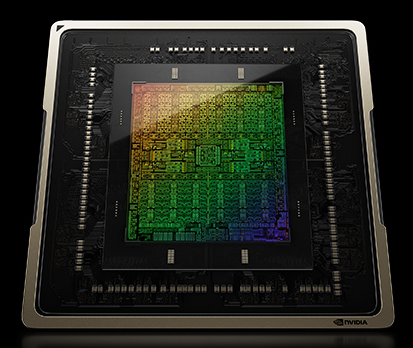
\includegraphics[width = 2.0in]{Screenshot 2023-08-21 190358.png}}
\caption{\textbf{NVIDIA Ada Lovelace Architecture}}
\label{figAM9300}
\end{figure}

 
\par À medida que a inteligência artificial e o processamento de vídeo continuam a se difundir amplamente, a necessidade por soluções de computação eficientes e econômicas está crescendo bastante. Esta GPU oferece um desempenho de vídeo em IA até 120 vezes superior, resultando em uma eficiência energética aprimorada em até 99\% e uma redução significativa nos custos totais de propriedade em comparação com as infraestruturas tradicionais baseadas em CPU. Isso permite que empresas otimizem o funcionamento de seus equipamentos, ao mesmo tempo em que expandem a capacidade de seus centros de dados para atender a um número significativamente maior de usuários.

\par Em relação a utilização desta placa no mercado, diversas empresas grandes a utilizam, como descript, Twitter, SnapChat e o Google Cloud.


\begin{figure}[h]
\centerline{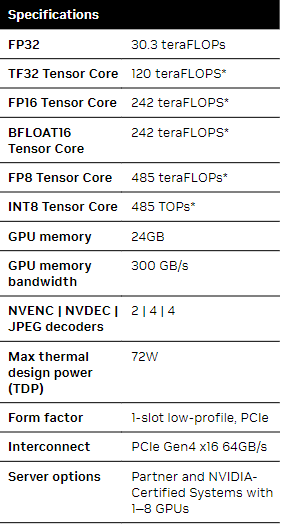
\includegraphics[width = 2.4in]{Screenshot 2023-08-19 230710.png}}
\caption{\textbf{Datasheet NVIDIA L4 Tensor Core}}
\label{figAM9300}
\end{figure}


\subsubsection{NVIDIA IGX Orin}

\par A NVIDIA IGX Orin representa uma plataforma de categoria industrial que integra elementos de hardware, software e suporte voltados para empresas. Essa plataforma integral e abrangente, a IGX, possibilita que as organizações direcionem seus esforços para o desenvolvimento de aplicativos, acelerando consideravelmente os ganhos provenientes da inteligência artificial.Seu módulo conta com uma CPU: 12-core ARM, GPU Ampere 1024 CUDA, 64 Tensor.


\begin{figure}[h]
\centerline{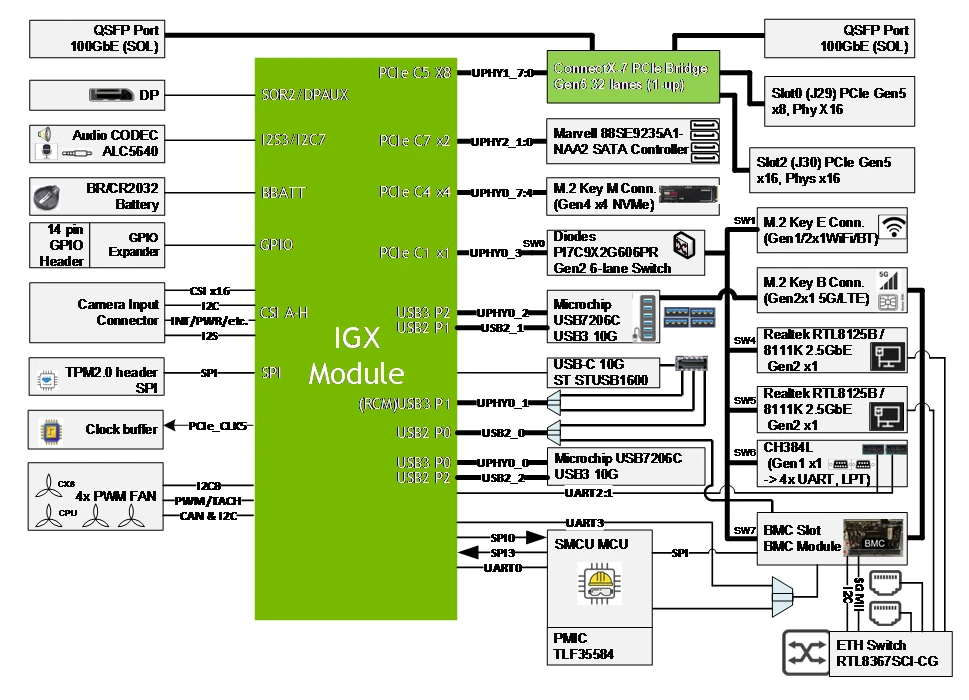
\includegraphics[width = 2.5in]{Screenshot 2023-08-21 191640.png}}
\caption{\textbf{IGX Module}}
\label{figAM9300}
\end{figure}


\par A NVIDIA IGX oferece capacidades grandes e seguras de computação, rede e software para aplicação na automação industrial e dispositivos médicos. A plataforma IGX abrange drivers compatíveis com sistemas operacionais comerciais, um pacote de extensão de segurança para programação de funções de segurança no sistema, e suporte empresarial de longo prazo abrangendo toda a pilha de software.

\par A concepção da NVIDIA IGX Orin tem como foco proporcionar um desempenho ultra-rápido que se encaixa perfeitamente nas dimensões e nas demandas de consumo de energia necessárias para aplicações de edge computing. Movido pelo mais avançado sistema de IA do mundo, que oferece incríveis 275 tera operações por segundo (TOPS) de desempenho em IA para máquinas autônomas eficientes em termos energéticos, o IGX Orin também integra uma placa de interface de rede inteligente NVIDIA ConnectX-7 (SmartNIC), garantindo precisão de temporização e recursos de segurança avançados.
Esta plataforma abrange ainda provisionamento e gestão remotos, bem como uma ilha funcional de segurança integrada e uma unidade de microcontrolador de segurança (sMCU), a qual pode ser programada através de extensões de software para proporcionar segurança preventiva em ambientes autônomos. Em suma, a NVIDIA IGX é intrinsecamente segura e protegida, fundamentada em seu próprio design.

\par Em relação ao seu uso, percebe-se que permiti a correlação entre máquinas e humanos tanto no meio industrial, quanto no meio médico, já que esta plataforma oferece eficiência e segurança, principalmente nestes meios, fazendo com que todo o âmbito de trabalho se torne um espaço inteligente de utilização, acelerando diversos processos e permitindo um grande aumento de eficiência.  

\par Em relação a utilização desta plataforma por algumas empresas e centros médicos, há alguns parceiros da NVIDIA, como Siemens, Canonical e Activ Surgical.


\begin{figure}[h]
\centerline{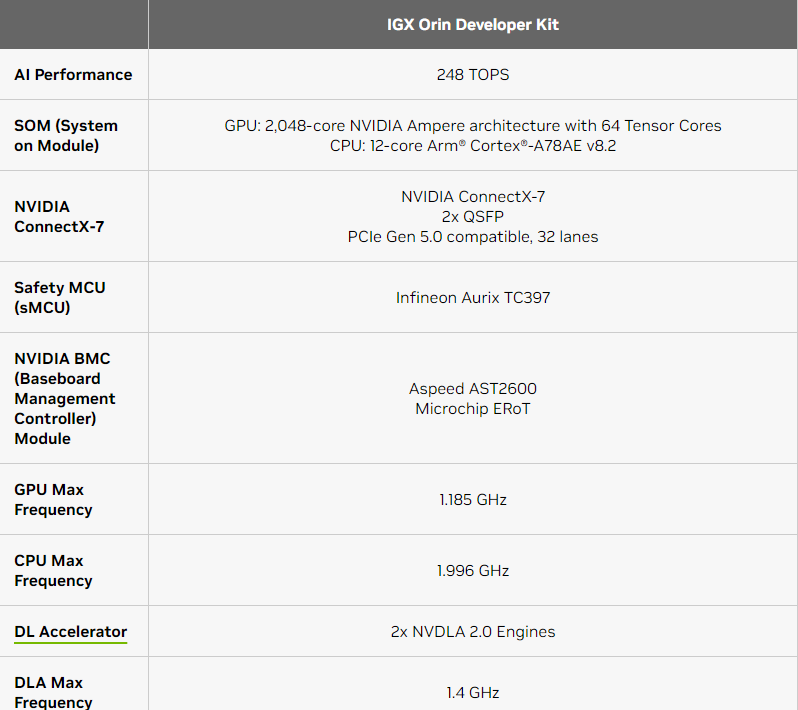
\includegraphics[width = 2.2in]{Screenshot 2023-08-20 000908.png}}
\caption{\textbf{Datasheet NVIDIA IGX Orin}}
\label{figAM9300}
\end{figure}

\begin{figure}[h]
\centerline{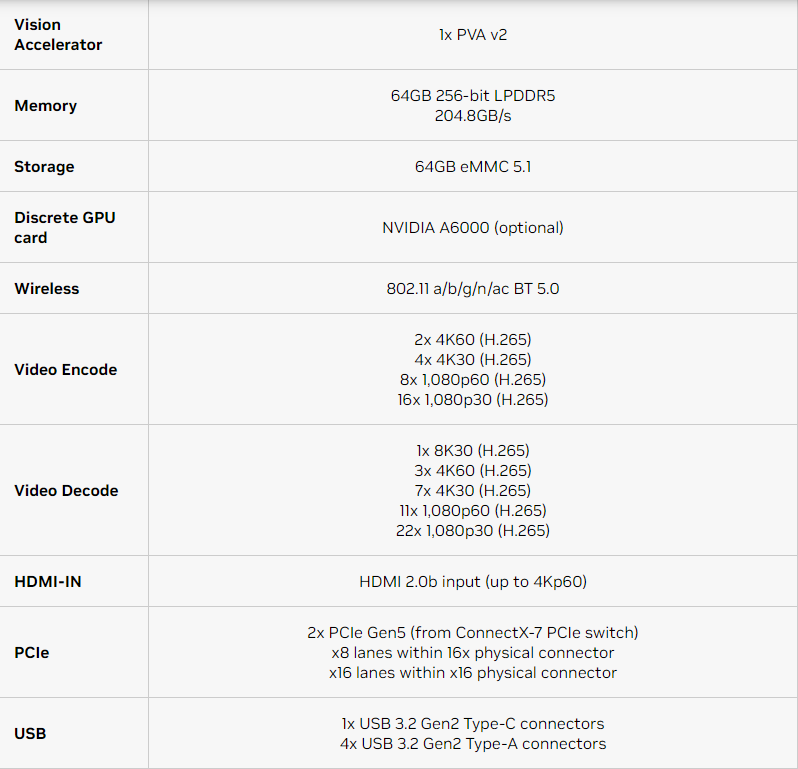
\includegraphics[width = 2.2in]{Screenshot 2023-08-20 000929.png}}
\caption{\textbf{Datasheet NVIDIA IGX Orin}}
\label{figAM9300}
\end{figure}



\begin{figure}[h]
\centerline{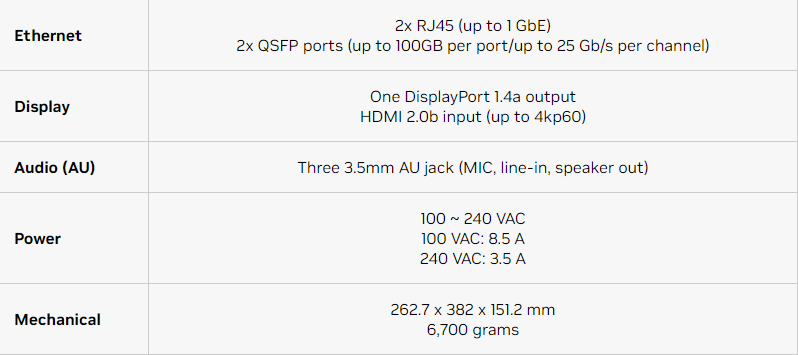
\includegraphics[width = 2.2in]{Screenshot 2023-08-20 000941.png}}
\caption{\textbf{Datasheet NVIDIA IGX Orin}}
\label{figAM9300}
\end{figure}


\subsection{No Mercado Aeroespacial}
\subsubsection{Introdução}

\par A adoção de produtos da NVIDIA no mercado aeroespacial representa um marco significativo na evolução tecnológica dessa indústria crucial. A NVIDIA tem desempenhado um papel fundamental ao fornecer soluções avançadas de computação gráfica, inteligência artificial e deep learning para o mercado aeroespacial. Com sua expertise em chips gráficos e hardware de alto desempenho, a NVIDIA estabeleceu sólidas parcerias com agências espaciais, como a NASA, para aprimorar a qualidade das simulações de voo e facilitar tarefas complexas, como navegação, monitoramento de missões e processamento de dados em tempo real. Esta colaboração não apenas eleva o padrão da experiência espacial, mas também destaca a importância da tecnologia de ponta na exploração e pesquisa fora da Terra.

\par Algumas das tecnologias que a NVIDIA forneceu para o mercado aeroespacial são: GPUs para simulações e treinamentos, GPUs para processamento de dados e análise, GPUs para sistemas de autonomia e inteligência artificial para aeronaves e satélites e sistemas de visão computacional.

\subsubsection{GPU NVIDIA Quadro RTX 8000}

\par A NVIDIA lançou a Quadro RTX 8000 em 13 de agosto de 2018 como uma placa de vídeo profissional destinada a entusiastas. Esta placa é construída com a tecnologia de processo de 12 nm e é baseada no processador gráfico TU102, especificamente a variante TU102-875-A1. Ela oferece suporte ao DirectX 12 Final. O chip TU102 é notável por sua grande área de matriz, com 754 mm² e uma impressionante quantidade de 18.600 milhões de transistores. A placa conta com 4608 unidades de sombreamento, 288 unidades de mapeamento de textura e 96 ROPs. Além disso, possui 576 núcleos tensores, que aceleram aplicativos de aprendizado de máquina, bem como 72 núcleos de aceleração de ray tracing.

\begin{figure}[h]
\centerline{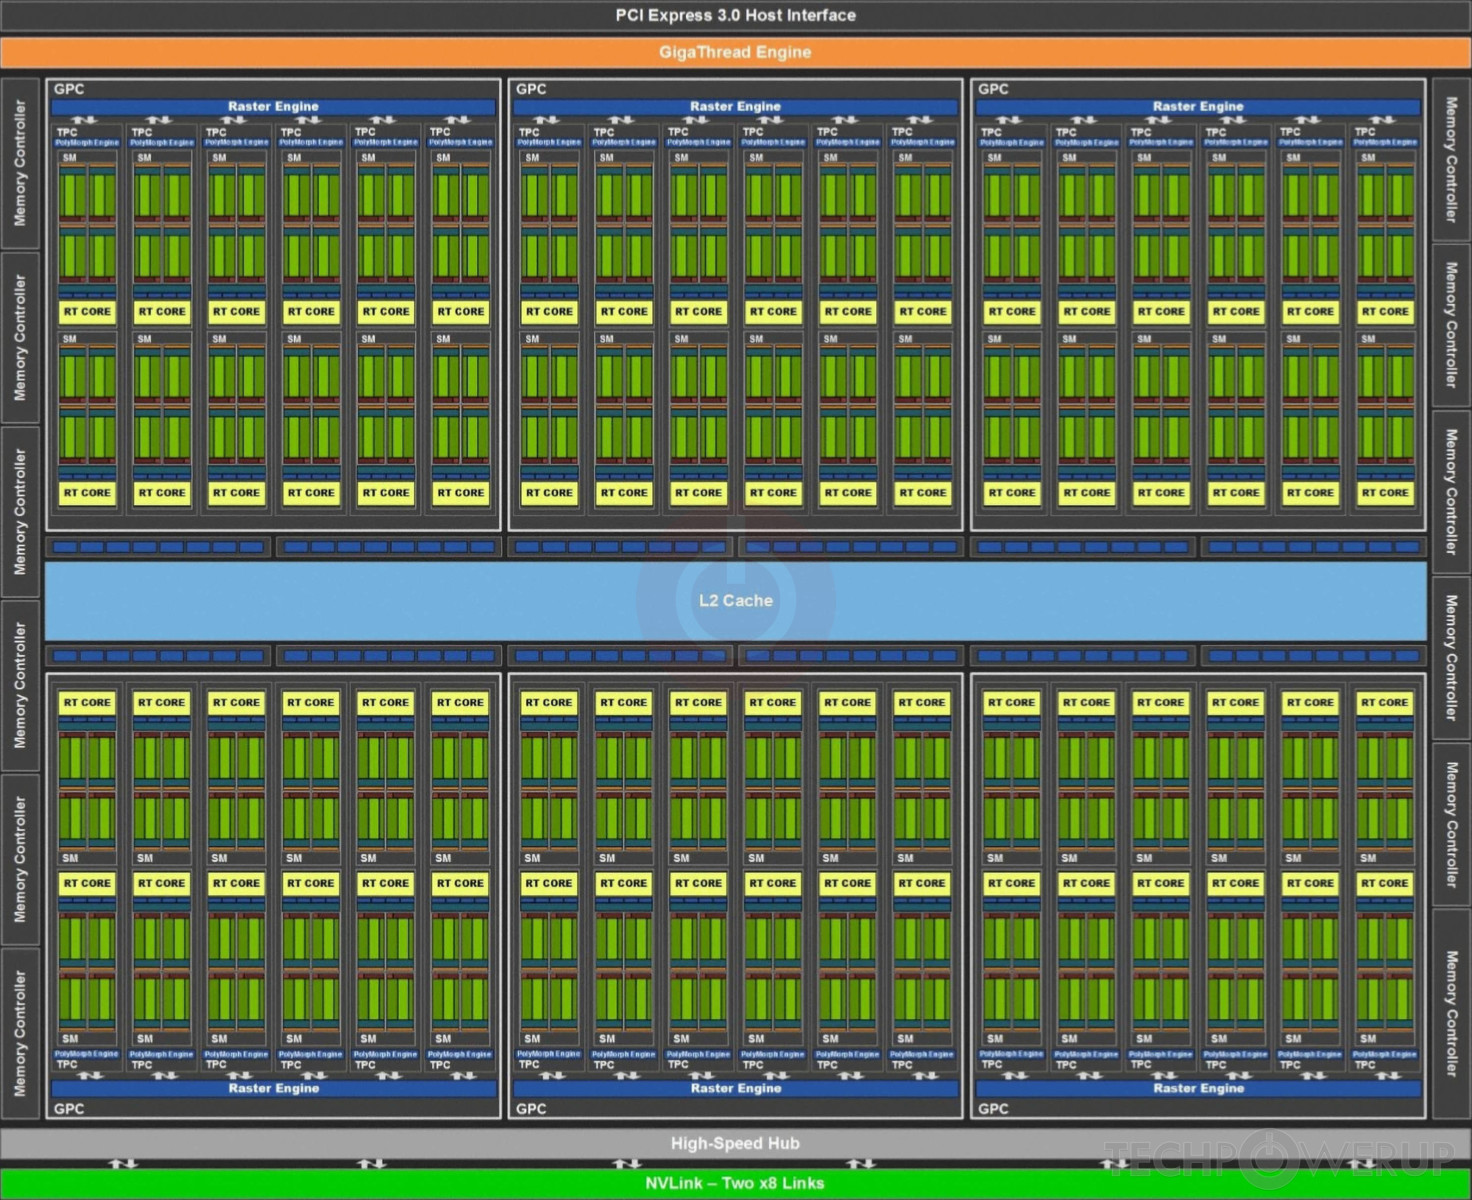
\includegraphics[width = 2.0in]{tu102.jpg}}
\caption{\textbf{Processador Gráfico - TU102}}
\label{figAM9300}
\end{figure}

\par A Quadro RTX 8000 é equipada com 48 GB de memória GDDR6 conectados através de uma interface de memória de 384 bits. A GPU tem uma frequência base de 1395 MHz, que pode ser aumentada para até 1770 MHz, enquanto a memória funciona a 1750 MHz (14 Gbps efetivos).

\par Em relação à alimentação, esta placa de dois slots requer um conector de alimentação de 6 pinos e um conector de 8 pinos, com um consumo máximo de energia avaliado em 260 W. As opções de saída incluem 4x DisplayPort 1.4a e 1x USB Type-C. A conexão com o sistema é feita por meio de uma interface PCI-Express 3.0 x16. A Quadro RTX 8000 possui dimensões de 267 mm de comprimento, 111 mm de largura e um sistema de resfriamento de slot duplo. Seu preço de lançamento foi de 9.999 dólares americanos.

\par Algumas utilizações da NVIDIA Quadro RTX 8000  na área aeroespacial são para simulações e treinamentos de piloto, análise de dados de satélites e missões espaciais. A NASA, por exemplo, encontrou essa placa como solução, por exemplo, para acelerar a análise de imagens solares coletadas pelo Solar Dynamics Observatory, uma sonda não-tripulada da NASA, com objetivo de estudar processos do sol que afetam diretamente a vida na Terra.

\begin{figure}[h]
\centerline{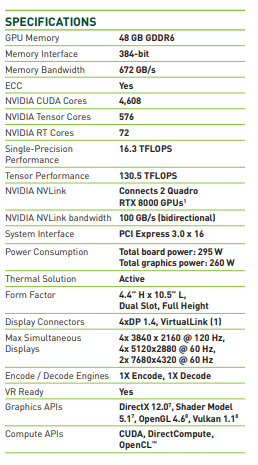
\includegraphics[width = 2.0in]{datasheet quadro rtx 8000.png}}
\caption{\textbf{Datasheet GPU NVIDIA Quadro RTX 8000}}
\label{figAM9300}
\end{figure}

\subsubsection{GPU NVIDIA A100 Tensor Core}

\par A placa de vídeo profissional da NVIDIA, conhecida como GPU Nvidia A100 Tensor Core, foi lançada em 16 de novembro de 2020. Ela utiliza o processo de fabricação de 7 nm e tem como base o processador gráfico GA100. Importante mencionar que esta placa não suporta o DirectX.

\par O processador gráfico GA100 é um chip consideravelmente grande, ocupando uma área de matriz de 826 mm² e contendo um número total de 54.200 milhões de transistores. Ele possui 6912 unidades de sombreamento, 432 unidades de mapeamento de textura e 160 ROPs. Além disso, inclui 432 tensor cores que têm o propósito de melhorar a velocidade das aplicações de aprendizado de máquina. A NVIDIA equipou a A100 80 GB com uma memória HBM2e de 80 GB, conectada através de uma interface de memória de 5120 bits. A GPU opera a uma frequência padrão de 1275 MHz, com capacidade de overclock de até 1410 MHz, enquanto a memória funciona a 1593 MHz.

\begin{figure}[h]
\centerline{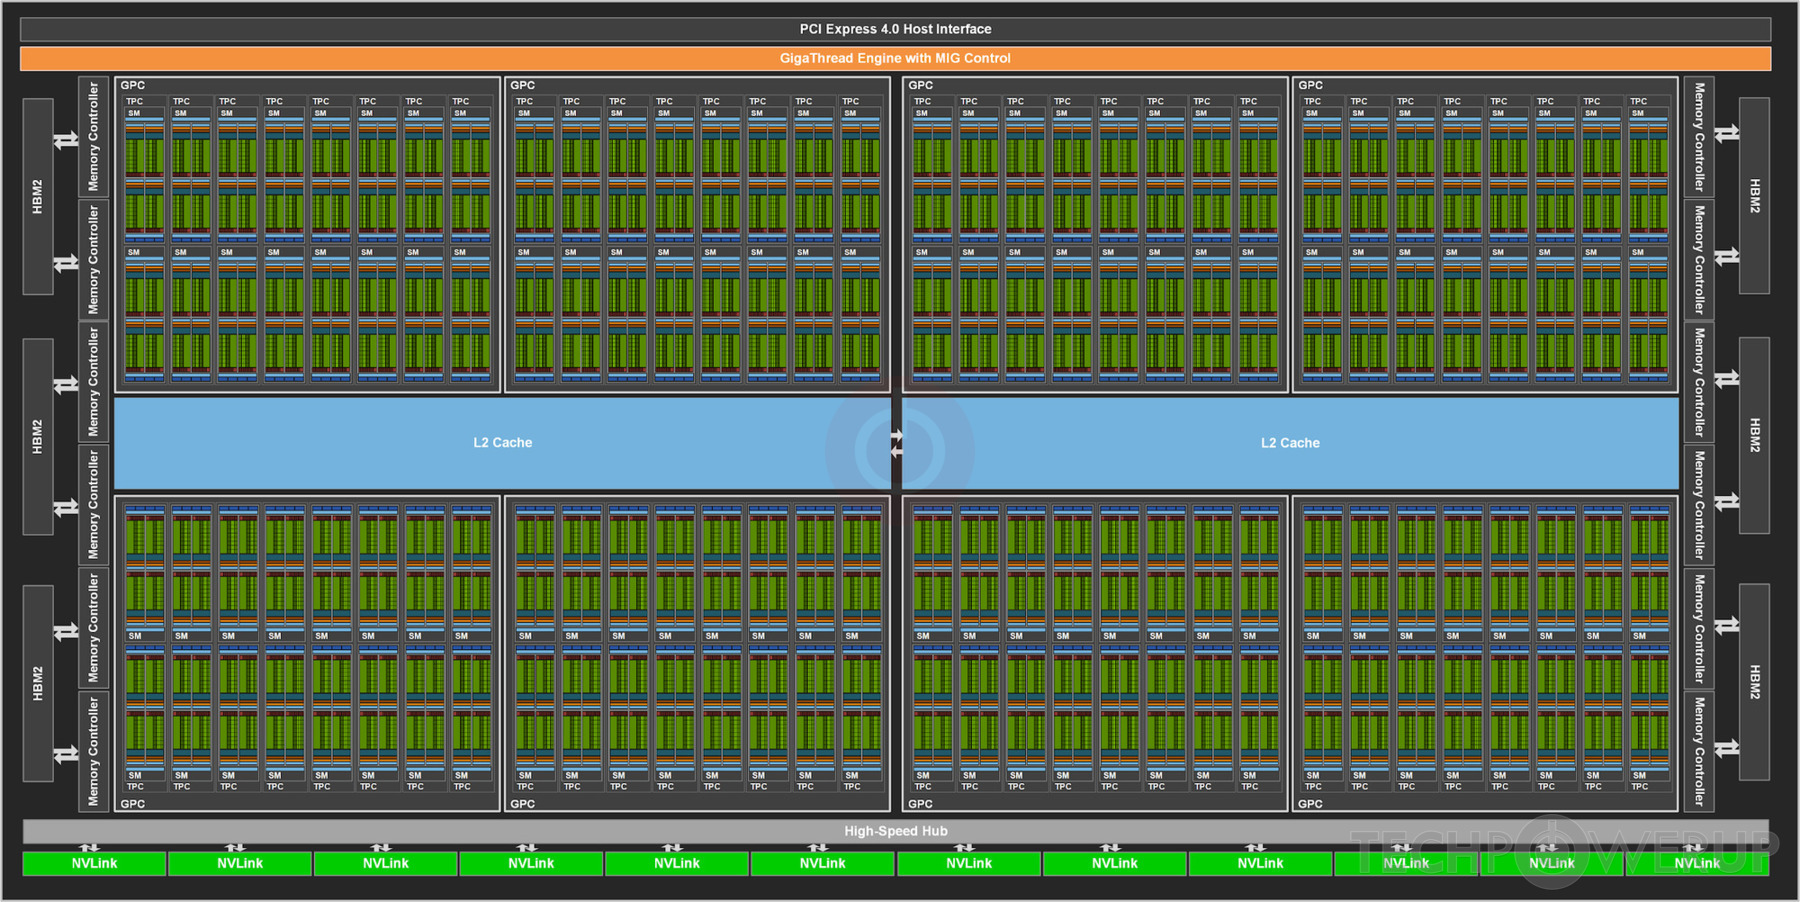
\includegraphics[width = 2.0in]{ga100.jpg}}
\caption{\textbf{Processador Gráfico - GA100}}
\label{figAM9300}
\end{figure}

\par Sendo uma placa de módulo OAM (On-Board Adaptive Module), a NVIDIA A100 80 GB não requer conectores de alimentação adicionais e tem um consumo máximo de energia avaliado em 400 W para o modelo SXM e 300 W para o modelo PCIe. É importante notar que esta placa não possui conectores para monitores, uma vez que não foi projetada para conexão direta a eles. A conexão com o resto do sistema é feita através de uma interface PCI-Express 4.0 x16.

\par Esta GPU proporciona aceleração em todas as escalas, impulsionando os data centers mais potentes do mundo dedicados à IA, análise de dados e HPC.  Alimentado pela Arquitetura NVIDIA Ampere, o A100 é o motor da plataforma de data center da NVIDIA. Esta placa gráfica oferece suporte a uma ampla gama de precisões matemáticas, fornecendo um único acelerador para cada carga de trabalho. A versão de última geração do A100, com 80 GB de memória, dobra a capacidade da GPU e apresenta a maior largura de banda de memória do mundo, atingindo 2 terabytes por segundo, acelerando assim o tempo de solução para os modelos e conjuntos de dados mais extensos.

\par A GPU NVIDIA A100 Tensor Core é amplamente adotada em aplicações aeroespaciais, devido aos ganhos significativos de desempenho que oferece em uma variedade de tarefas computacionais. Ela possibilita simulações mais ágeis e precisas, processamento de imagem e sinal, aprendizado de máquina e computação de alto desempenho, tornando-a extremamente relevante para aplicações na área aeroespacial. Uma das empresas que incorporou com este produto da NVIDIA é a Silicon Mechanics, que oferece sistemas de GPU personalizados, incluindo soluções voltadas para a indústria aeroespacial.

\begin{figure}[!h]
\centerline{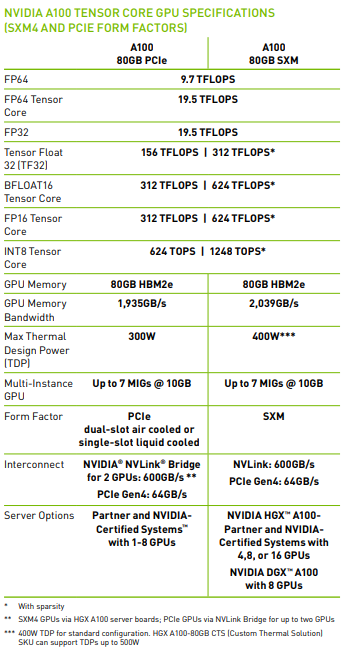
\includegraphics[width = 2.0in]{datasheet a100 tensor core.png}}
\caption{\textbf{Datasheet GPU NVIDIA A100 Tensor Core}}
\label{figAM9300}
\end{figure}

\subsection{No Mercado Militar}
\subsubsection{Introdução}
\par A NVIDIA tem alguns produtos próprios para o mercado militar, porém as informações sobre o que ela produz de cunho militar é um pouco escasso, pois são informações poderosas. Contudo sabe-se que a NVIDIA trabalha com algumas empresas do ramo militar, por exemplo a General Dynamic: que é um conglomerado de empresas de defesa americano. No ano de 2008 tornou-se a quinta maior empresa do setor de Defesa no mundo. A empresa é baseada em Falls Church, no estado da Virgínia. Outra empresa que se tem registro que trabalha junto com ela é a Lockheed Martin: é uma empresa fabricante de produtos aeroespaciais criada em 1995, resultante da fusão da Lockheed Corporation e da Martin Marietta. Está sediada em Bethesda, Maryland, uma comunidade no Condado de Montgomery.
\par Um exemplo de aplicação direta das placas de vídeo da empresa no contexto militar foi uma tecnologia desenvolvida em uma parceria com a NVIDIA e com a DARPA que é o braço tecnológico do exército americano no que diz respeito aos objetos e tecnologias mais incríveis que existem, A tecnologia chama Virtual Eye, que basicamente une duas imagens em um ambiente 3D em tempo real. Isso é feito com o auxílio de um notebook poderoso e duas câmeras, podendo assim fazer com que o soldado veja o que existe atrás de parede e de obstáculos. E o notebook em questão roda duas GPUs NVIDIA K20.

\subsubsection{GPU NVIDIA A40 PCIe}
\par A A40 PCIe é uma placa de vídeo profissional da NVIDIA, lançada em 5 de outubro de 2020. Construída no processo de 8 nm e baseada no processador gráfico GA102, a placa suporta DirectX 12 Ultimate. O processador gráfico GA102 é um chip grande com uma área de matriz de 628 mm² e 28.300 milhões de transistores. Possui 10752 unidades de sombreamento, 336 unidades de mapeamento de textura e 112 ROPs. Também estão incluídos 336 núcleos tensores que ajudam a melhorar a velocidade dos aplicativos de aprendizado de máquina. A placa também possui 84 núcleos de aceleração de raytracing. 

\begin{figure}[h]
\centerline{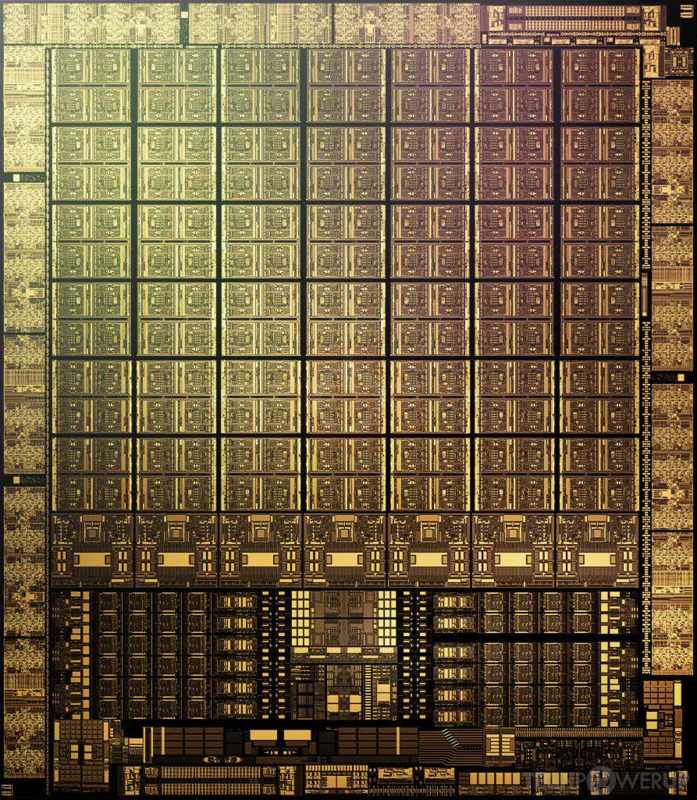
\includegraphics[width = 1.7in]{a40_imagem.jpg}}
\caption{\textbf{Processador gráfico GA102}}
\label{figAM9300}
\end{figure}

\par A NVIDIA combinou 48 GB de memória GDDR6 com o A40 PCIe, que são conectados usando uma interface de memória de 384 bits. A GPU está operando a uma frequência de 1305 MHz, que pode ser aumentada até 1740 MHz, a memória está operando a 1812 MHz (14,5 Gbps efetivos).
\par Sendo uma placa de dois slots, a NVIDIA A40 PCIe consome energia de um conector de alimentação EPS de 8 pinos, com consumo de energia avaliado em 300 W no máximo. As saídas de vídeo incluem: 3x DisplayPort 1.4a. A40 PCIe é conectado ao resto do sistema usando uma interface PCI-Express 4.0 x16. A placa mede 267 mm de comprimento, 111 mm de largura e possui uma solução de resfriamento de slot duplo.



\begin{figure}[h]
\centerline{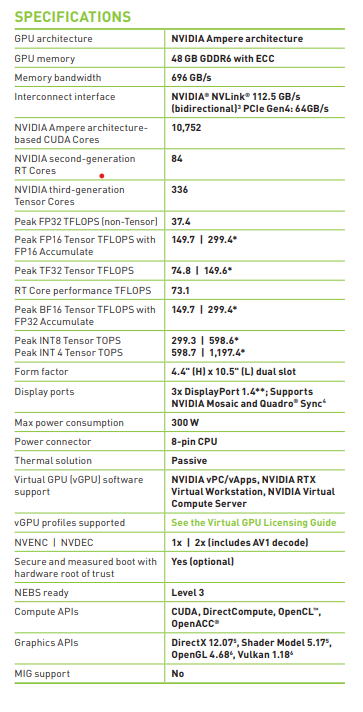
\includegraphics[width = 2.0in]{dataa40.png}}
\caption{\textbf{GPU Nvidia A40 PCIe}}
\label{figAM9300}
\end{figure}

\subsubsection{GPU NVIDIA Tesla K20X}
\par A Tesla K20X era uma placa de vídeo profissional para entusiastas da NVIDIA, lançada em 12 de novembro de 2012. Construída no processo de 28 nm e baseada no processador gráfico GK110, a placa suporta DirectX 12. O processador gráfico GK110 é um chip grande com uma área de matriz de 561 mm² e 7.080 milhões de transistores. Possui 2688 unidades de sombreamento, 224 unidades de mapeamento de textura e 48 ROPs.

\begin{figure}[h]
\centerline{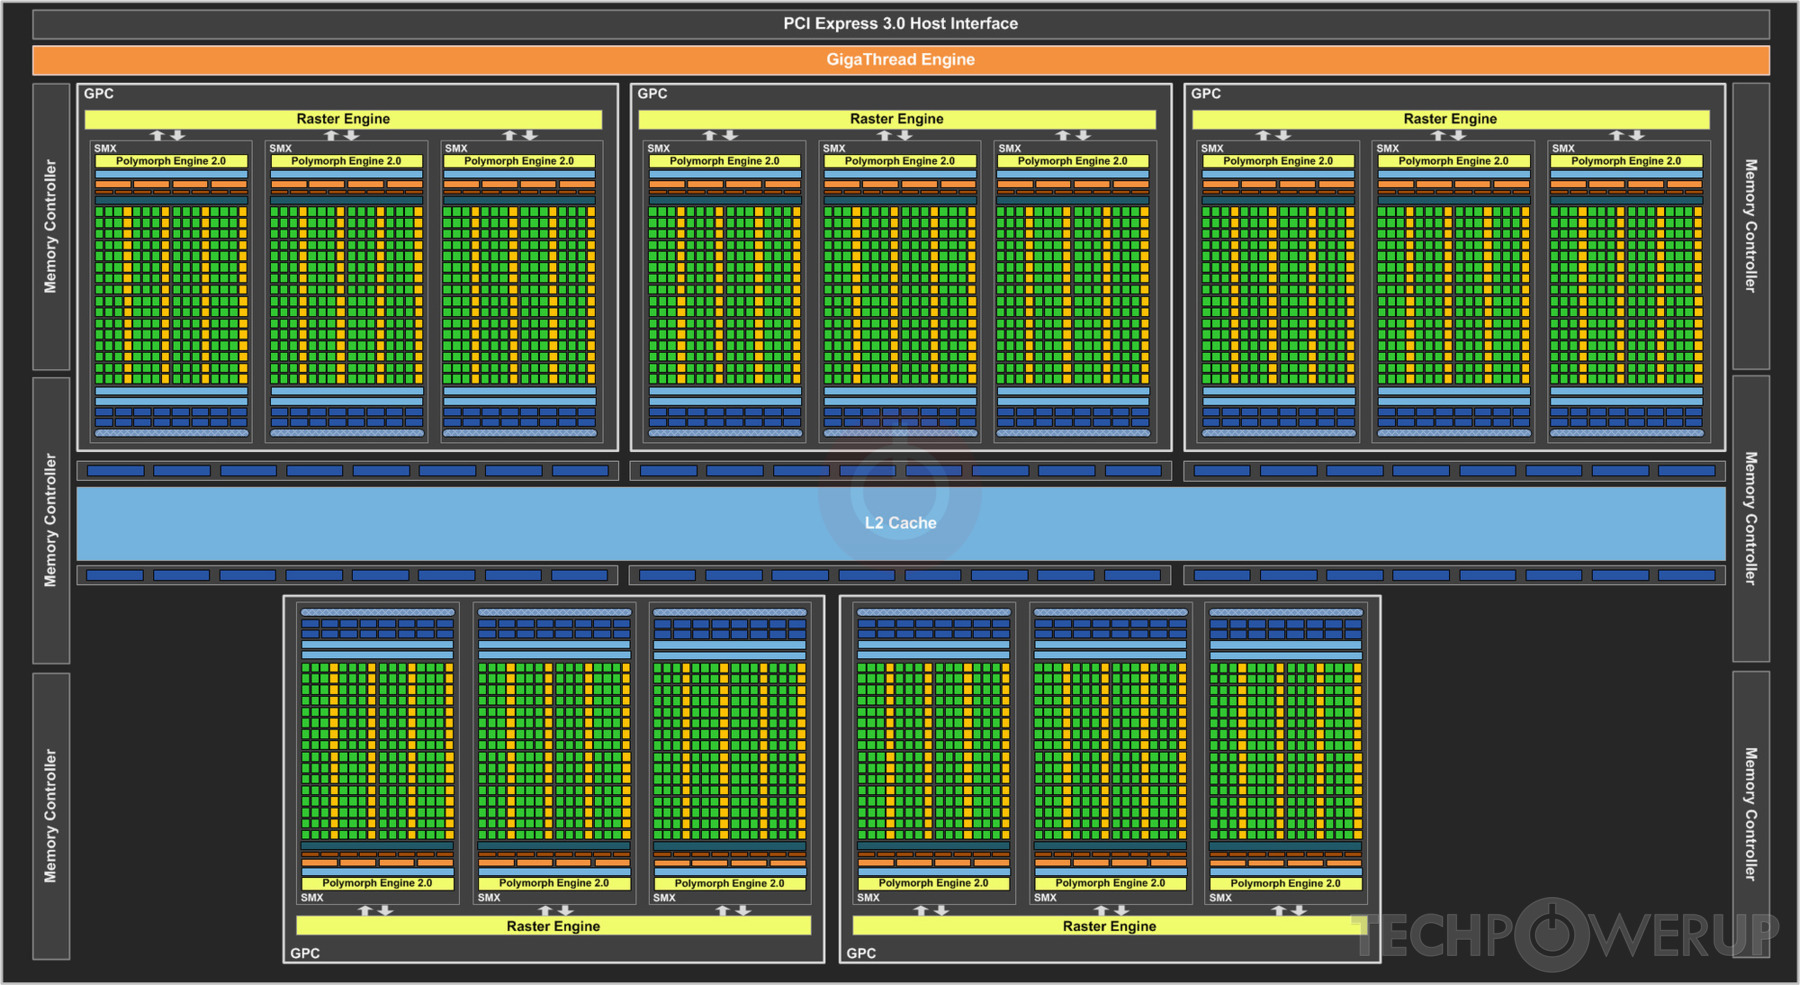
\includegraphics[width = 2.0in]{nvidia gk110.jpg}}
\caption{\textbf{Processador Gráfico GK110}}
\label{figAM9300}
\end{figure}

\par A NVIDIA combinou 6 GB de memória GDDR5 com o Tesla K20X, que são conectados usando uma interface de memória de 384 bits. A GPU está operando a uma frequência de 732 MHz, a memória está funcionando a 1300 MHz (5,2 Gbps efetivos).
\par Sendo uma placa de dois slots, a NVIDIA Tesla K20X consome energia de 1 conector de alimentação de 6 pinos + 1 conector de 8 pinos, com consumo de energia avaliado em 235 W no máximo. Este dispositivo não possui conectividade de monitor, pois não foi projetado para ter monitores conectados a ele. O Tesla K20X está conectado ao resto do sistema usando uma interface PCI-Express 3.0 x16. A placa mede 267 mm de comprimento e possui uma solução de resfriamento de slot duplo. Seu preço no lançamento era de 7.699 dólares americanos.

\begin{figure}[!h]
\centerline{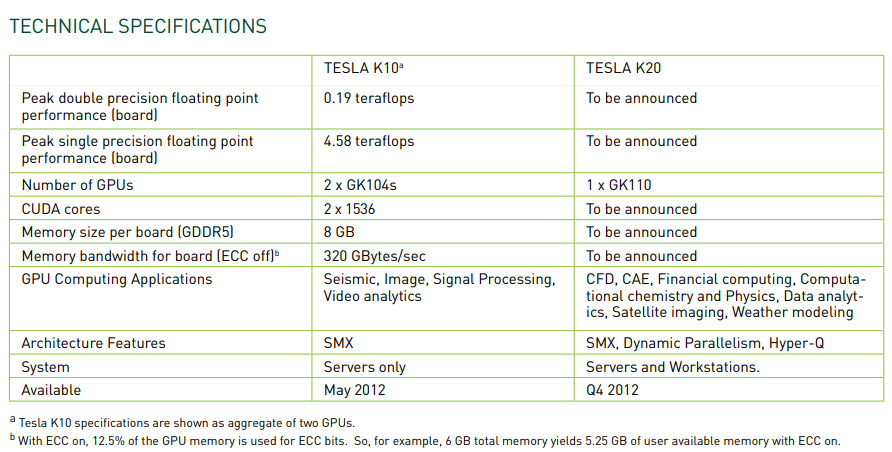
\includegraphics[width = 3.4in]{datak20.png}}
\caption{\textbf{Datasheet GPU NVIDIA Tesla K20x}}
\label{figAM9300}
\end{figure}

\subsubsection{GPU NVIDIA Tesla C2050}
\par A Tesla C2050 foi uma placa gráfica profissional da NVIDIA, lançada em 25 de julho de 2011. Construída no processo de 40 nm, e baseada no processador gráfico GF100, em sua variante GF100-850-A3, a placa suporta DirectX 12. A GF100 O processador gráfico é um chip grande com uma área de matriz de 529 mm² e 3.100 milhões de transistores. Ao contrário da GeForce GTX 480 Core 512 totalmente desbloqueada, que usa a mesma GPU, mas tem todos os 512 shaders ativados, a NVIDIA desativou algumas unidades de sombreamento no Tesla C2050 para atingir a contagem de shaders alvo do produto. Possui 448 unidades de sombreamento, 56 unidades de mapeamento de textura e 48 ROPs. A NVIDIA combinou 3.072 MB de memória GDDR5 com o Tesla C2050, que são conectados usando uma interface de memória de 384 bits. A GPU está operando a uma frequência de 574 MHz, a memória está funcionando a 750 MHz (3 Gbps efetivos).
Sendo uma placa de dois slots, a NVIDIA Tesla C2050 consome energia de 1 conector de alimentação de 6 pinos + 1 conector de 8 pinos, com consumo de energia avaliado em 238 W no máximo. As saídas de exibição incluem: 1x DVI. O Tesla C2050 está conectado ao resto do sistema usando uma interface PCI-Express 2.0 x16. A placa mede 248 mm de comprimento e possui uma solução de resfriamento de slot duplo.

\begin{figure}[h]
\centerline{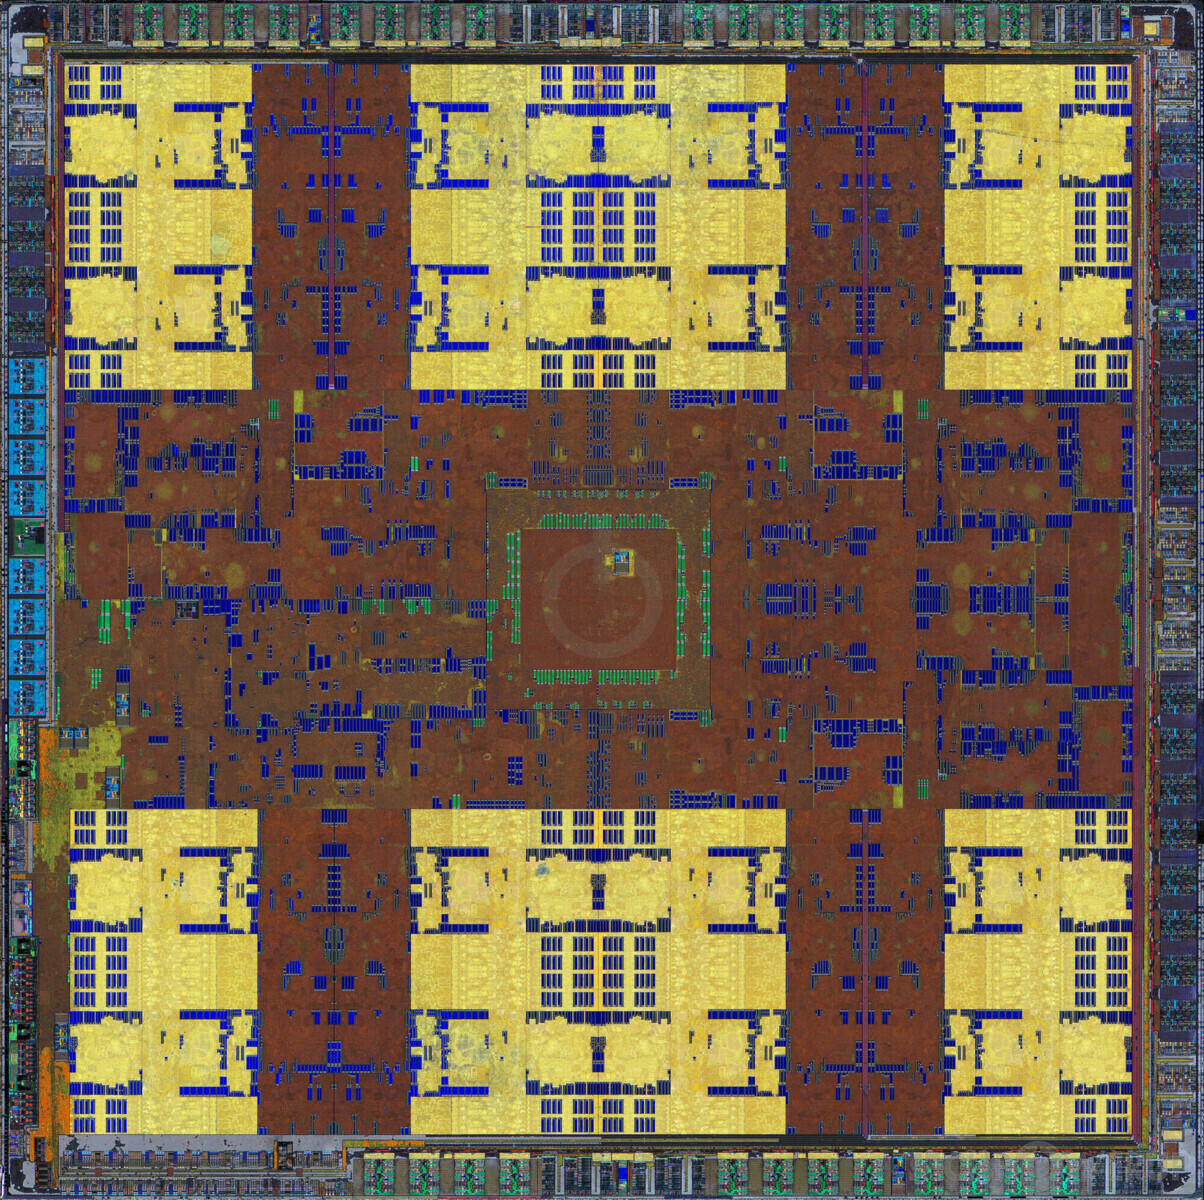
\includegraphics[width = 2.0in]{85-die-shot.jpg}}
\caption{\textbf{GPU NVIDIA Tesla c2050}}
\label{figAM9300}
\end{figure}

\begin{figure}[!h]
\centerline{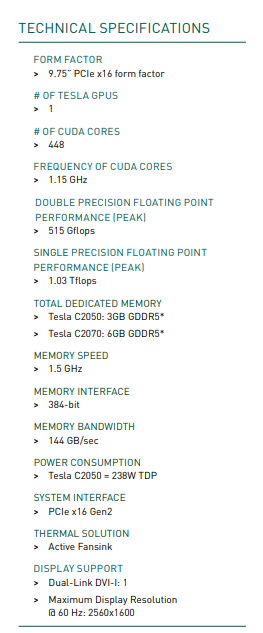
\includegraphics[width = 2.0in]{datac2050.png}}
\caption{\textbf{Datasheet GPU NVIDIA Tesla c2050}}
\label{figAM9300}
\end{figure}

\section{Mercado}
\subsection{Introdução}
\par Segundo a categorização descritiva do relatório das receitas referentes ao terceiro trimestre de 2021, divulgados pela própria Nvidia, a empresa de chips atende a cinco expressivos mercados: indústria automotiva, jogos, data center, fabricação de equipamentos originais (da sigla em inglês, OEM[Original Equipment Manufacturer]) e visualização profissional, todos envolvendo a área de IA, que, juntamente com a questão de processamento gráfico, representa a área de maior destaque da empresa.

\subsection{Impacto financeiro de cada mercado}
\par Seguidamente, no que refere-se ao impacto das estreitas relações comerciais com esses mercados no caixa da empresa, adotando como referencial o relatório citado anteriormente, o mercado de jogos corresponde a 45\% da receita líquida total, seguido do mercado de data center, com 41\%, o segmento de visualização profissional, com 8\%, a indústria automotiva, com 2\%, e a fabricação de equipamentos originais, com 3\%.

\subsection{Descrição dos segmentos de mercado presente no trabalho}
\par Com o fito de dar um enfoque maior nos segmentos de mercado referentes ao mercado industrial, aeroespacial e militar, na sequência, as relações da Nvidia com cada segmento será descrita, sob uma perspectiva de análise mercadológica e comercial.

\par Inicialmente, no que se refere à atuação da Nvidia no desenvolvimento de produtos e soluções, em termos de hardware e software, com empresas que atuam no setor industrial, alguns dos segmentos supracitados apresentam expressivo destaque. Dentre eles, a indústria automotiva.

\subsection{Indústria automotiva}
\par No que diz respeito a indústria automotiva, a Nvidia possui relações acuradas e expressivas com grandes players desse setor, sendo esses: Mercedes-Benz, Jaguar, Volvo, Hyundai Motor Group, Foxconn, etc.
\par Adotando uma perspectiva mais específica e pragmática, acerca de como essas parcerias comerciais com esse setor da indústria se dão, ressalta-se a existência dos seguintes campos de atuação da Nvidia no setor supracitado: 

\begin{figure}[h]
\centerline{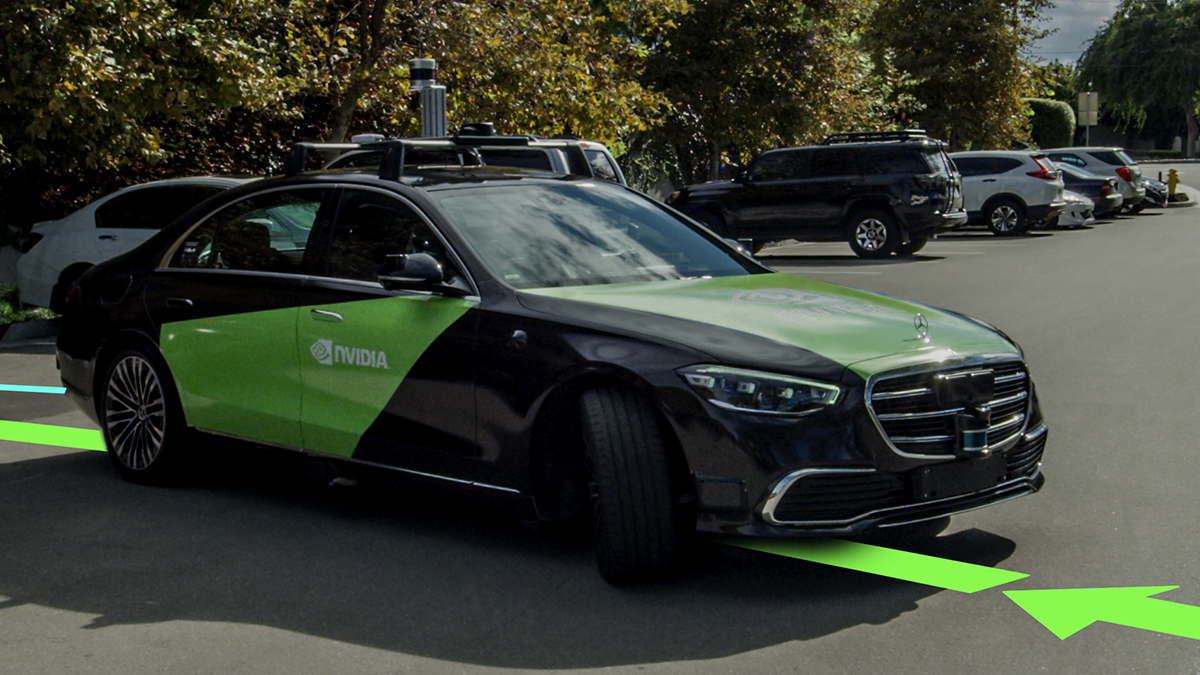
\includegraphics[width = 3.0in]{automovel.jpg}}
\caption{\textbf{Carro, da montadora Mercedes-Benz, com sistema Nvidia Drive}}
\label{figAM9300}
\end{figure}

\par \textbf{Plataformas de Processamento Automotivo:} A Nvidia empreende o desenvolvimento de múltiplas plataformas de computação automotiva, destaca-se o NVIDIA DRIVE, em parceria com as empresas supracitadas, para a composição de sistemas avançados de assistência ao motorista (ADAS) e automóveis autônomos. De modo geral, essas plataformas, utilizando IA e hardware de processamento específico para a mesma, processam os dados produzidos por sensores, presentes no projeto do automóvel, e auxiliam na tomada de decisão na direção.

\par \textbf{Desenvolvimento de Aplicações e Simulação:} Atualmente, a Nvidia disponibiliza variadas ferramentas de desenvolvimento de software e simulação prática de testes, que estão sendo amplamente utilizadas no processo produtivo das montadoras, a fim de, por meio de modelos de deep learning aplicados nesse processo de construção e efetivação de testes, validar todas as etapas composicionais da cadeia produtiva. 

\par \textbf{Automação veicular: }Presentemente, a Nvidia, em conjunto com as montadoras, empregam a construção de sistemas de direção autônoma, em que o mesmo é incumbido de processar dados, provenientes dos múltiplos sensores, e, por meio de modelos de deep learning, tomar decisões de modo proativo e seguro, em tempo real. O principal produto da empresa, nesse segmento, corresponde a plataforma NVIDIA DRIVE.

\subsection{Fabricação (OEM)}
\par Além da indústria automotiva, a Nvidia, atua fortemente como Original Equipment Manufacturer (fabricante de equipamentos originais), em que a mesma integra as cadeias de produção de diversos setores, dentre eles, estão os setores requisitados pelo vigente trabalho: militar, aeroespacial e industrial, em que a Nvidia compõe, por meio de soluções em hardware e/ou software, uma expressiva cadeia produtiva.

\par Primeiramente, vale expor as empresas, de múltiplos mercados (inclusive industrial, aeroespacial e militar), que a Nvidia já compôs ou compõe a cadeia produtiva de seus produtos originais(sendo esses, soluções de hardware e/ou software) Lenovo, Acer, RED Digital Cinema, Siemens (\textbf{mercado industrial} - software de simulação e design 3D), Boeing (\textbf{mercado aeroespacial} - simulação e treinamento para pilotos), Northrop Grumman (\textbf{mercado militar e aeroespacial} - processamento de dados voltados à aplicações militares e aeroespaciais), Raytheon Technologies (\textbf{mercado militar e aeroespacial} - sistema de radar avançado de rastreamento e detecção).

\par Na sequência, vale ressaltar que essa atuação confere a Nvidia um papel expressivo e estratégico no mercado, evidenciando a relevância e primazia atrelados à empresa.

\par Seguidamente, tem-se que a Nvidia opera sob múltiplas estratégias e abordagens no mercado de OEM, sendo essas:


\par \textbf{Fornecimento de plataformas de desenvolvimento:} A Nvidia empreende o desenvolvimento de múltiplas plataformas que servem, de um modo geral, como base para composição de sistemas mais complexos e específicos. Um exemplo disso é o supracitado NVIDIA DRIVE, que é utilizado por montadoras para a construção de seus próprios sistemas de assistência de direção ou direção autônoma.


\par \textbf{Produção de componentes-chaves:} A Nvidia provê múltiplos componentes essenciais que são integrados às versões finais dos produtos das empresas parceiras. Em termos de hardware, essa relação se dá por meio de hardware especializado em processamento de inteligência artificial e GPUs, aplicadas em múltiplos produtos, do mais básico e simples, como um desktop pessoal, ao mais complexo e custoso, como um sistema de IA para detecção de objetos voadores, em um contexto militar. Já em termos de software, essa relação está lastreada nas plataformas de desenvolvimento supracitados.


\par \textbf{Criação de ecossistemas:} A Nvidia, ao compor a cadeia produtiva de múltiplos setores que fabricam vários produtos, dispõe e utiliza do ambiente ideal para uma criação e difusão de ecossistemas tecnológicos abrangentes, em que, ao integrar seu hardware e/ou software à outros produtos, promove os mais variados “pontos comuns” que servem como base para a integração entre esses produtos.

\subsection{\textbf{Visualização profissional}} 
A mais de 20 anos a Nvidia possui ampla atuação na área de computação visual profissional, quando se diz a respeito de aplicativos profissionais relacionados com  Manufatura, Imagens médicas e científicas e Energia até Mídia e entretenimento, através dos modelos de placa de video “Quadro”, que utiliza de tecnologias avançadas de visualização que visa proporcionar a melhor experiência visual e aumento considerável de produtividade em workflows.

Na sequência, vale ressaltar que a Nvidia mantém relações com múltiplas empresas , de diversos setores, na área de computação visual profissional. Dentre essas empresas destacam-se:
\begin{itemize}[h]
    \item Lockheed Martin (\textbf{setor militar} - projetos de simulação e visualização avançados para práticas militares)
    \item General Dynamics (\textbf{setor militar}  - sistemas de análise de risco e monitoramento de campo)
    \item Rockwell Automation (\textbf{setor industrial} - sistema de análise e gestão de processos industriais)
\end{itemize}

As Placas de vídeo “Quadro”, suportam displays de 4K e Ultra HD, podem expandir facilmente o espaço de exibição para vários monitores simultâneos e realizar exibição com visão 3D estereoscópica imersiva.

\begin{figure}[h]
\centerline{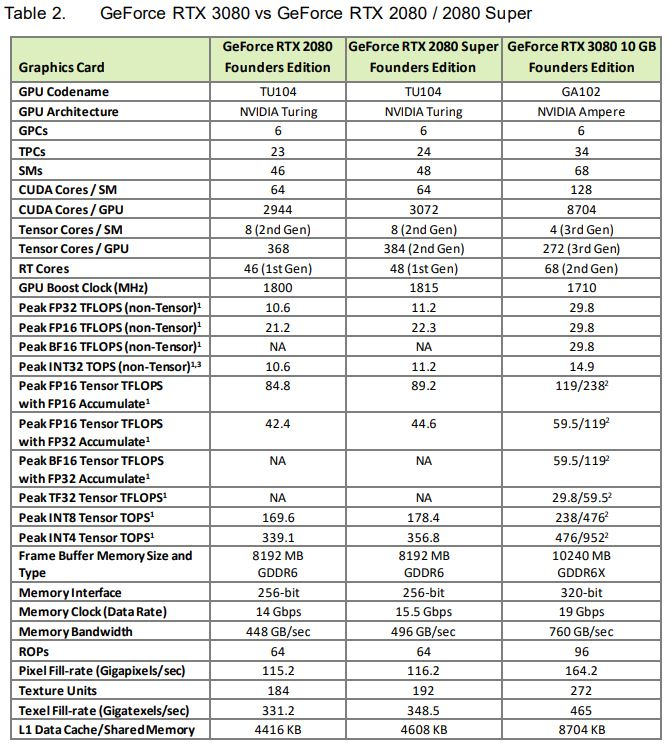
\includegraphics[width = 3.0in]{tabelafodase.jpg}}
\caption{\textbf{Datasheet: NVIDIA Ampere GA102 GPU Architecture}}
\label{figAM9300}
\end{figure}

\begin{figure}[h]
\centerline{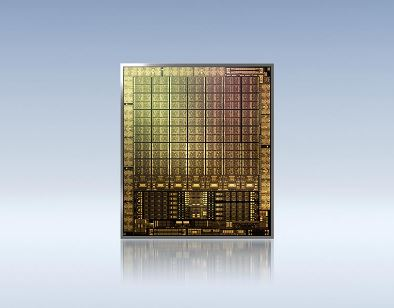
\includegraphics[width = 3.0in]{chipfodase.JPG}}
\caption{\textbf{Chip: Arquitetura Ampere}}
\label{figAM9300}
\end{figure}

\subsection{\textbf{Data Center}}  A Nvidia sempre foi fundamental na indústria de Data center com suas tecnologias avançadas. Eles oferecem alternativas para que as diversas empresas possam lidar com grande quantidade de dados.

A Nvidia é indiscutivelmente líder no mercado de aceleração de GPU, Sua arquitetura “Ampere” se destaca no mercado por conta de seu desempenho superior e eficiência energética. E como as empresas estão se adaptando a inteligência artificial e incorporando-a cada vez mais em suas operações, por causa disso,A NVIDIA posiciona suas soluções como impulsionadoras cruciais para IA e aprendizado de máquina, com suas GPUs acelerando o treinamento e inferência de modelos complexos. Isso ressoa especialmente com empresas que buscam insights profundos de dados para tomar decisões estratégicas informadas.

Em resumo, a Nvidia se destaca no mercado de data center por oferecer múltiplas soluções de aceleração de GPU, impulsionar a inovação em inteligência artificial, otimizar a eficiência operacional e atender às demandas de processamento de alta performance. Sua presença dominante e seu compromisso com a inovação tecnológica fazem da NVIDIA uma escolha lógica para empresas que buscam vantagens competitivas através de recursos avançados de processamento e análise de dados.

\section{Conclusão}
\par Com a realização desse trabalho, aprendemos mais sobre a NVidia, uma empresa que faz-se muito presente no dia a dia de muitos usuários de computadores. Mas ao invés de aprendermos mais sobre o que está sempre em grande visibilidade na mídia, como seu produtos voltados para \textit{gamers}, foi possível descobrir sobre mercados fora dos triviais nos quais ela tem/teve participação.
\par Dessa forma, por mais que não seja tão simples encontrar informações sobre a empresa nos ramos fora de jogos eletrônicos e inteligência artificial, visto que foge do \textit{mainstream}, foi possível realizar toda a pesquisa sem grandes complicações, uma vez que a empresa tem um alcance global e um grande nome no mercado.
\par Ademais, foi possível aprender um pouco mais sobre o funcionamento de equipamentos similares ao que possuímos em nossos computadores ou de pessoas próximas.

\begin{thebibliography}{00}

\bibitem{b1} ‌4-datasheet-2595652.pdf. Widen.net. Disponível em: <https://nvdam.widen.net/s/rvq98gbwsw/l4-datasheet-2595652>. Acesso em: 17 ago. 2023.
\bibitem{b2} AYÃO, Felipe. Tecnologia militar permite que soldados vejam atrás de obstáculos. Tecmundo.com.br. Disponível em: <https://www.tecmundo.com.br/tecnologia-militar/106543-tecnologia-militar-permite-soldados-vejam-obstaculos.htm>. Acesso em: 17 ago. 2023.
\bibitem{b3} CASTRO, Nicole. NASA’s Day in the Sun: Space Agency Speeds Analysis of Solar Images by 150x Using Data Science Workstations | NVIDIA Blog. NVIDIA Blog. Disponível em: <https://blogs.nvidia.com/blog/2020/06/18/nasa-data-science-workstations/>. Acesso em: 17 ago. 2023.
\bibitem{b4} DUBOVSKIY, John. Nvidia Marketing Strategy Overview - Research-Methodology. Research-Methodology. Disponível em: <https://research-methodology.net/nvidia-marketing-strategy-overview/>. Acesso em: 17 ago. 2023.
\bibitem{b5} GLOBALDATA PLC. NVIDIA Corp Company Profile - NVIDIA Corp Overview. Globaldata.com. Disponível em: <https://www.globaldata.com/company-profile/nvidia-corp/>. Acesso em: 17 ago. 2023.
\bibitem{b6} GOEL, Shikhar. What does Nvidia do: Business model analysis. The Strategy Story. Disponível em: <https://thestrategystory.com/2023/01/05/what-does-nvidia-do-business-model-analysis/>. Acesso em: 17 ago. 2023.
\bibitem{b7} KAGAN, Julia. Original Equipment Manufacturer (OEM): Definition and Examples. Investopedia. Disponível em: <bit.ly/45VBEwX>. Acesso em: 17 ago. 2023.
\bibitem{b8} NVIDIA A100 GPUs Power the Modern Data Center. NVIDIA. Disponível em: <https://www.nvidia.com/en-us/data-center/a100/>. Acesso em: 17 ago. 2023.
\bibitem{b9} NVIDIA A100 SXM4 80 GB Specs. TechPowerUp. Disponível em: <https://www.techpowerup.com/gpu-specs/a100-sxm4-80-gb.c3746>. Acesso em: 17 ago. 2023.
\bibitem{b10} NVIDIA A40 PCIe Specs. TechPowerUp. Disponível em: <https://www.techpowerup.com/gpu-specs/a40-pcie.c3700>. Acesso em: 17 ago. 2023.
\bibitem{b11} NVIDIA Announces Financial Results for First Quarter Fiscal 2024. Nvidia.com. Disponível em: <https://investor.nvidia.com/news/press-release-details/2023/NVIDIA-Announces-Financial-Results-for-First-Quarter-Fiscal-2024/default.aspx>. Acesso em: 17 ago. 2023.
\bibitem{b12} NVIDIA Corporation: History. NVIDIA. Disponível em: <https://www.nvidia.com/en-us/about-nvidia/corporate-timeline/>. Acesso em: 17 ago. 2023.
\bibitem{b13} NVIDIA IGX Platform. NVIDIA. Disponível em: <https://www.nvidia.com/en-us/edge-computing/products/igx/#get-started>. Acesso em: 17 ago. 2023.
\bibitem{b14} NVIDIA L4 Specs. TechPowerUp. Disponível em: <https://www.techpowerup.com/gpu-specs/l4.c4091>. Acesso em: 17 ago. 2023.
\bibitem{b15} NVIDIA Quadro RTX 8000 Specs. TechPowerUp. Disponível em: <https://www.techpowerup.com/gpu-specs/quadro-rtx-8000.c3306>. Acesso em: 17 ago. 2023.
\bibitem{b16} NVIDIA TU102 GPU Specs. TechPowerUp. Disponível em: <https://www.techpowerup.com/gpu-specs/nvidia-tu102.g813>. Acesso em: 17 ago. 2023.
\bibitem{b17} NVIDIA. AI da NVIDIA para o Setor Automotivo. NVIDIA. Disponível em: <https://www.nvidia.com/pt-br/industries/automotive/>. Acesso em: 17 ago. 2023.
\bibitem{b18} NVIDIA. AI solutions for industrial applications | NVIDIA. NVIDIA. Disponível em: <https://www.nvidia.com/pt-br/industries/industrial/>. Acesso em: 17 ago. 2023.
\bibitem{b19} NVIDIA. Design e Visualização Profissionais NVIDIA. NVIDIA. Disponível em: <https://www.nvidia.com/pt-br/design-visualization/>. Acesso em: 17 ago. 2023.
\bibitem{b20} NVIDIA. Our Body of Work. [s.l.: s.n., s.d.]. Disponível em: <https://images.nvidia.com/aem-dam/Solutions/homepage/pdf/NVIDIA-Story.pdf>. Acesso em: 17 ago. 2023.
\bibitem{b21} NVIDIA. Parceiros NVIDIA Drive. NVIDIA. Disponível em: <https://www.nvidia.com/pt-br/self-driving-cars/partners/>. Acesso em: 17 ago. 2023.
\bibitem{b22} PARTNERBASE. Partners of NVIDIA. Partnerbase.com. Disponível em: <https://www.partnerbase.com/nvidia>. Acesso em: 17 ago. 2023.
\bibitem{b23} Previous Generation Desktop Graphics Cards from NVIDIA Quadro. NVIDIA. Disponível em: <https://www.nvidia.com/pt-br/design-visualization/previous-quadro-desktop-gpus/>. Acesso em: 17 ago. 2023.
\bibitem{b24} REIFF, Nathan. How Nvidia Makes Money: Graphics Segment Generates the Most Revenue. Investopedia. Disponível em: <https://www.investopedia.com/how-nvidia-makes-money-4799532>. Acesso em: 17 ago. 2023.
\bibitem{b25} SAUNDERS, Amanda. New NVIDIA IGX Platform Helps Create Safe, Autonomous Factories of the Future | NVIDIA Blog. NVIDIA Blog. Disponível em: <https://blogs.nvidia.com/blog/2022/09/20/igx-industrial-edge-ai/>. Acesso em: 17 ago. 2023.
\bibitem{b26} SCIENCE X. Nvidia chip team gets 25 million dollars from US military. Phys.org. Disponível em: <https://phys.org/news/2010-08-nvidia-chip-team-million-dollars.html>. Acesso em: 17 ago. 2023.
\bibitem{b27} ‌Silicon Mechanics Powers High-Performance Workloads in Aerospace and Defense Industry with NVIDIA GPUs. HPCwire. Disponível em: <https://www.hpcwire.com/off-the-wire/silicon-mechanics-powers-high-performance-workloads-in-aerospace-and-defense-industry-with-nvidia-gpus/>. Acesso em: 17 ago. 22023.
\bibitem{b28} TECMUNDO. A história da NVIDIA! História da Tecnologia. Disponível em: <https://www.youtube.com/watch?v=xKlmCikZun8\&ab\_channel=TecMundo>. Acesso em: 17 ago. 2023.
\bibitem{b29} The Most Powerful Compute Platform for Every Workload NVIDIA A100 TENSOR CORE GPU Unprecedented Acceleration at Every Scale NVIDIA A100 TENSOR CORE GPU SPECIFICATIONS (SXM4 AND PCIE FORM FACTORS). [s.l.: s.n., s.d.]. Disponível em: <https://www.nvidia.com/content/dam/en-zz/Solutions/Data-Center/a100/pdf/nvidia-a100-datasheet-nvidia-us-2188504-web.pdf>.Acesso em: 17 ago. 2023.
\bibitem{b30} US Navy gets 8.2 petaflops supercomputer. Datacenterdynamics.com. Disponível em: <https://www.datacenterdynamics.com/en/news/us-navy-gets-82-petaflops-supercomputer/>. Acesso em: 17 ago. 2023.
\bibitem{b31} VIDIA L4 Tensor Core GPU. NVIDIA. Disponível em: <https://www.nvidia.com/pt-br/data-center/l4/>. Acesso em: 17 ago. 2023.
\bibitem{b32} YAHOO FINANCE. NVIDIA Corporation (NVDA) Stock Price, News, Quote \& History - Yahoo Finance. @YahooFinance. Disponível em: <https://finance.yahoo.com/quote/NVDA/>. Acesso em: 17 ago. 2023.

\end{thebibliography}
\vspace{12pt}

\end{document}
